\mysection{Wizardry}{arcana-wizardry}

\flavor{[B]lood aids great sorcery!" thundered Xaltotun, in a voice that made the rocks quiver \Tilde R.E.H., "The Hour of the Dragon"}

The arcana of Wizardry are powered through blood; to manifest a spell you must roll one or more of your Blood Dice - how many is up to you, but you have to roll them all at once.  Each Blood Die is a \POOL, meaning if you roll a \myital{natural} 1 or a 2, you lose the die. 

Rolling 3 dice or more carries an additional risk:

\mybullet {
  \item If you roll any triples, roll on the \mylink{Mishap table}{table-mishap}. The spell works.
  \item If you roll any quadruples, roll on the \mylink{Calamity table}{table-calamities}. The spell fails.
  \item If you roll any quintuples, roll on the \mylink{Ruin table}{table-ruin}. The spell fails.  This will most likely kill you.
}

You restore 1 Blood Die when you take a \mylink{Bivouac}{combat-resting-bivouac}.  You restore \myital{all} your Blood Die during a Vacation.  If you are out of Blood, you can attempt to ride \mybold{the Torrent}


\mysubsection{The Torrent}{philosopher-torrent}

If you have 0 Blood Dice in your pool, you can try to cast your Wizardry arcana directly from the Torrent (a dangerous proposition).  For each Blood Die you want to add to your Wizardry, try the following \RO:

\example {
  \mybold{Torrent}

  \RO : \INT plus d6 plus Modifiers ~\\ ~\\

  \myital{Don't forget to add your \LVL, since this roll uses your \INT!}
}

If you succeed, you can add a Blood Die to the spell.  You can do this as many times as you like for each spell. If you fail any \RO attempt, the spell fails and you suffer a \mylink{Calamity}{table-calamities}.

  \begin{center}
  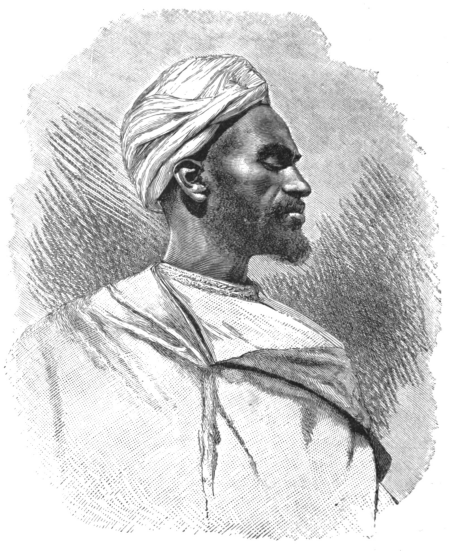
\includegraphics[scale=.5]{Philosopher_1}
  \end{center}


\mysubsection{Components}{philosopher-components}

If you have the \mylink{Virtue: Crux of Blood}{philosopher-virtue-blood}, you can harvest and use components to cast spells:

\example {
  \mybold{Harvest Component}
  \RO : \INT plus d6 plus d20 plus Modifiers

  ~\\
  
  \myital{Don't forget to add your \LVL, since this roll uses your \INT!}
}

If you succeed on your \RO try, gain d4 \UD of a Component.

You decide what Components augment which spells. For example, you could declare that kobold's eyes are a component for the spell Sleep.  If you succeed in your \RO try, then kobold's eyes are always a component for Sleep (note it on your character sheet) for YOU and not for anyone else (someone else's version of Sleep has a different way of casting, needs boggart boogers or whatever). 

If you cast a spell with a Component, then you only burn a Blood die if you roll a 1 (instead of a 1 or 2).  Components are Insignificant items, but using a component consumes it in a puff of smoke / blue flame / swarm of gnats etc.

\mybullet {
  \item Components can only be harvested during a Breather, and have to be from one of the Monsters you've (presumably) killed.  It has to be something you can reasonably carry (Arbiter's choice) - basilisk tongue, OK.  Green slime, not OK.
  \item Monsters only provide one component.  You can't say kobold's eyes help Magic Missile and kobold's tongues help cast Battering Beam.   
  \item You can only try once per Monster type per Breather, so if you kill 9 kobolds and 14 trolls then you get two shots - once on kobolds and once on trolls.
  \item You can only harvest d4 \UD from a Monster no matter how many there are - 9 kobolds or 1, you get d4 \UD
}


\mysubsection{Grimoires}{philosopher-grimoires}

Grimoires are solid, with thick vellum pages and a sturdy cover. Special runes and symbols trap spells inside cages of crystallized thought. Each book contains enough room for 10 spells. Some spells must be stored across several pages for safety, so the books contain more than 10 pages, and have
plenty of room for notes, ledgers, or sketches - and curses, hexes, coded and cryptic entries written with poisonous and hallucinogenic inks. Grimoires start in a waterproof, acid- and fire-resistant bag. Outside the bag, they are not waterproof and are quite flammable. See the section on
\mylink{Inscription}{research-inscription} for more details.


\mysubsection{Fetishes}{philosopher-fetishes}

Fetishes are inscribed with a single spell from your Grimoire, cranium, or another fetish.  All fetishes have a \UD of d4 - when the \UD is exhausted, the magical words disappear from the fetish.  A Sorcerer's skull counts as a fetish, though obviously the brain can't be in the way if you want to read
it.  See the section on \mylink{Inscription}{research-inscription} for more details.

You may cast the spell from the Fetish with any number of Blood you choose, OR you may forgo the Blood die and roll a single d6 for the effect.

\cbreak

\mysubsection{Wizards' Duel}{philosopher-wizards-duel}

Certain spells can be countered by other spells - for example,
\mylink{Balthazar's Breathtaking
Blast}{wizardry-balthazars-breathtaking-blast} can be countered by
\mylink{Mighty Lungs}{wizardry-mighty-lungs}, and
\mylink{Invisibility}{wizardry-invisibility} can be dispelled by the wisps
summoned in the \mylink{Fool's Fire}{wizardry-fools-fire} spell. 

If you attempt to counter a spell and the Sorcerer who cast it is not
present (that is, not somewhere Close, Nearby, Far-Away, or Distant) you
automatically succeed.  Otherwise, you enter into a duel with the other
Sorcerer.

Each Sorcerer must \RB : \INT, adding their \LVL and the \DICE invested in
the spell as well as any other modifiers.  

\example {
  \mybold{A Wizards' Duel is}
  \RB : \INT plus \LVL plus \DICE
}


The winner's spell stays, the loser's spell goes.  Put another way: 

\mybullet{
  \item If you are countering a spell and you win, the spell you're
attempting to counter is dispelled and your spell takes effect
  \item If you are countering a spell and you lose, the spell you're
attempting counter remains and your spell fizzles with no effect.
}

If you attempt to counter a spell and you roll a \mylink{Calamity}{table-calamities} or \mylink{Ruin}{table-ruin}, the counterspell doesn't work. 


\newpage



\SPELL[
  Name=Acid Arrow,
  Link=wizardry-acid-arrow,
  Paradigm=Elements,
  Save=N,
  Duration=0/Markovian,
  Counter=None,
  Keywords=None,
  Target=Nearby or Far-Away Monster or Object
]

You throw an acidic arrow at a Monster or object. You must make a successful Fight check using your \INT (instead of \VIG or \DEX).  If you succeed: 

\mynumlist {
  \item If the target is wearing Armor, they must make a \UD check at the start of every Moment for the Markovian duration of the spell.  If they are using a shield, they may immediately sunder it to nullify the spell; 
  \item If they are not wearing Armor, they must take \DICE additional damage at the start of every Moment for the Markovian duration of the spell; 
  \item If the target is an object, it will melt a \DICE x 10cm cubic area of wood, metal, or stone.  
}

\SPELL[
  Name=Arcadia's Bulwark,
  Link=wizardry-arcadias-bulwark,
  Paradigm=Mind,
  Save=N,
  Duration=Session,
  Counter=\mylink{Acid Arrow}{wizardry-acid-arrow},
  Keywords=None,
  Target=Self
]


A spectral shield with a heraldic device of your choosing appears in the vicinity of your non-dominant arm.  The shield moves on its own to block Throw and Shoot weapons, and can absorb up to \SUMDICE + \DICE damage before it dissipates.  You can also Sunder this shield (like the Combat ability),
which also causes it to dissipate. You can still cast spells while this shield is summoned.  An Acid Arrow fired into the shield will dispel it if a Wizards' Duel is lost.


\SPELL[
  Name=Balthazar's Breathtaking Blast,
  Link=wizardry-balthazars-breathtaking-blast,
  Paradigm=Biomancy,
  Save=Y (negate),
  Duration=Markovian,
  Counter=\mylink{Mighty Lungs}{wizardry-mighty-lungs} ,
  Keywords=None,
  Target=Nearby or Far-Away point
]

A marble-sized bead of shit lands at a Nearby or Far-Away point you select. You can cause the sphere to detonate at any time in \DICE Hours (including immediately). All creatures Close or Nearby the sphere's detonation must
Save or immediately become Sickened, and the area is filled with a thick green mist that lasts for \DICE Hours.  Any who enter the mist during this time must Save or become Sickened, though you smell it and see it before
you're in it, so you won't stumble into it blindly.  Animals will avoid the area for the Markovian duration.  The spell does not affect creatures with no sense of smell, mindless creatures, or creatures who habitually live in
filth (goblins, shambling mounds, etc.).  The mist can be dispelled by Mighty Lungs if a Wizards' Duel is lost.




\SPELL[
  Name=Bastogne's Glamping Charm,
  Link=wizardry-bastognes-glamping-charm,
  Paradigm=Force,
  Save=N,
  Duration=Bivouac,
  Counter=\mylink{Morass}{wizardry-morass} ,
  Keywords=None,
  Target=Close
]



In an area you designate, a magical camp appears where you and \DICE-1 allies can Bivouac. The camp includes a bedroll, a sleeping platform, a small purple and gold tent, a small table and chair, a kettle, a cookpot
with a stew going, an iron arm to hold the kettle or cookpot over a fire, a book entitled "The Erotic Poems of Plumtarch" (less erotic than expected), and a pair of dry wool socks for up to \DICE people. Any items removed from
the area vanish instantly. In the spell's area, the temperature is moderated very slightly, wind and rain are lessened, and vermin cannot enter.  The tents are immune to casual attack, including from wandering Monsters (anyone
sleeping outside the tents might not be so lucky).  Up to \DICE people staying at the camp can forego a single Provisions \UD roll during their Bivouac.  The campsite can be utterly dispelled by Morass if a Wizards' Duel
is lost.

\SPELL[
  Name=Battering Beam,
  Link=wizardry-battering-beam,
  Paradigm=Force,
  Save=N,
  Duration=Concentration,
  Counter=\mylink{Battering Beam}{wizardry-battering-beam},
  Keywords=Contested,
  Target=Close or Nearby Monster or Object
]


A beam of force erupts from your forehead and strikes something you can see, pushing it backwards. Every Moment, the creature or object is pushed 5m in the direction you are looking.  If it's an object, you can push up to \DICE
x100kg.  If it's a creature, they can try to \RB: \VIG with a -\DICE penalty to fight back. If you lose the \RB try, the spell immediately ends - otherwise, the spell lasts as long as you concentrate. 
If the target cannot move backwards, it takes \DICE damage.  The Battering Beam can be dispelled by another Battering Beam if a Wizards' Duel is lost.




\SPELL[
  Name=Cacaphony,
  Link=wizardry-cacaphony,
  Paradigm=Entropy,
  Save=Y (negate),
  Duration=Varies,
  Counter=\mylink{Negasonic Bomb}{wizardry-negasonic-bomb} ,
  Keywords=None,
  Target=Nearby or Far-Away point
]



You roll a small orb of Entropy to a point Nearby or Far-Away; the orb rolls silently and is hard to see.  At any time for the next \SUMDICE Hours, you can have the orb detonate into an incredibly loud clattering, wailing, and
whistling. Creatures Close to the designated point must Save or be Stunned for \DICE Moments. It is audible in clear air up to a \DICE km away. You can designate \DICE conditions under which the orb will detonate. For example,
you could say "now"; "if anyone steps on it"; or "if water touches it".  The conditions must be obvious and must occur within 1m of the orb. When the spell's duration expires, you can choose to have the orb detonate (as above)
or vanish silently.  The Cacaphony can be dispelled by a Negasonic Bomb if a Wizards' Duel is lost.





\SPELL[
  Name=Charm,
  Link=wizardry-charm,
  Paradigm=Mind,
  Save=Y (negate),
  Duration=Session,
  Counter=\mylink{Charm}{wizardry-charm} ,
  Keywords=Contested,
  Target=Close Monster(s)
]



Ensorcel one or more Monsters whose combined \HD is less than or equal to \DICE.  Save negates; otherwise, they will regard you as a good friend and ignore the obvious spell you just cast on them.  The effect lasts for the
entire Session unless you ask them to do something they might think was a little weird: attack an ally, let you through an area they're supposed to be guarding, etc. (this is up to the Arbiter's discretion).  This prompts a
\RB: \FOC try with a -\DICE penalty.  You must touch the target's flesh (like with a handshake) to cast the spell.  The charmed person must stay Close, Nearby, or Far-Away from you - if you ever move beyond this distance, the spell is ended.  
The Charm can be broken and dispelled by another Charm if a Wizards' Duel is lost. 

  \begin{center}
  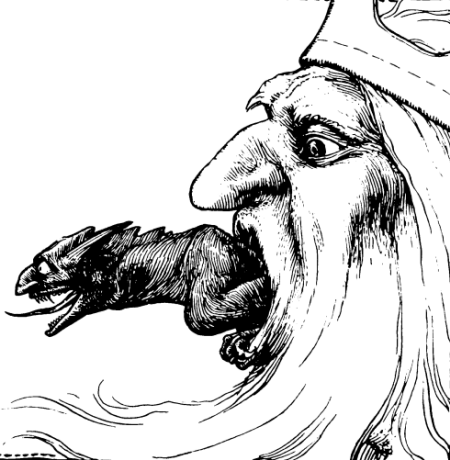
\includegraphics[scale=.5]{Tongue}
  \end{center}


\SPELL[
  Name=Color Spray,
  Link=wizardry-color-spray,
  Paradigm=Mind,
  Save=Y (negate),
  Duration=0 / Markovian,
  Counter=None ,
  Keywords=Splittable,
  Target=Close or Nearby Monster(s)
]



You emit \DICE sprays of color from your fingertips that you can split among \DICE Monsters.  For each Monster, if the \SUMDICE of the \DICE targeting the Monster is twice as much (equal to or greater) as the Monster's \HD, it
is Befuddled (the duration is Markovian and depends on the number of dice invested).  If \SUMDICE is three times the Monster's \HD, it is Stunned for a Moment, then Befuddled as above. If \SUMDICE is five times the creature's
\HD, it is Stunned (the duration is Markovian and depends on the number of dice invested), then Befuddled (Markovian duration).  Save negates.





\SPELL[
  Name=Commanding Presence,
  Link=wizardry-commanding-presence,
  Paradigm=Mind,
  Save=N,
  Duration=Combat or \SUMDICE Minutes,
  Counter=\mylink{Balthazar's Breathtaking Blast}{wizardry-balthazars-breathtaking-blast} ,
  Keywords=None,
  Target=Self
]

You grow +\DICE meters in height, and your features and voice become terrible and commanding.  Creatures of less than \DICE \HD must test morale or flee in terror.  You can use your \INT in place of any rolls where you
would normally use \VIG.  If you enter the radius of Balthazar's Breathtaking Blast, or if the spell is cast Close to you, the Commanding Presence is dispelled if a Wizards' Duel is lost.




\SPELL[
  Name=Ego Weapon,
  Link=wizardry-ego-weapon,
  Paradigm=Mind,
  Save=N,
  Duration=Session,
  Counter=\mylink{Greaseball}{wizardry-greaseball} ,
  Keywords=None,
  Target=Self
]



You can summon a Bashing, Cutting, or Stabbing weapon of Force.  You can change the type of weapon by using 1 Maneuver in Combat.  The weapon does \DICE damage and can hit creatures only affected by magic.  Only you can fight with the Ego Weapon.   You must make a successful
Fight check using your \INT (instead of \VIG or \DEX) to hit with the weapon.  A Helping Hand can wield an Ego Weapon, but you can only have 1 Ego Weapon in existence at a time.  The weapon lasts for the entire Session.  It can be dispelled by a Greaseball if a Wizards' Duel is lost; it will dispel an
Illusion spell with a touch if a Wizards' Duel is won.

\SPELL[
  Name=Enervate,
  Link=wizardry-enervate,
  Paradigm=Entropy,
  Save=Y (half),
  Duration=0,
  Counter=None ,
  Keywords=None,
  Target=Close or Nearby Magical Monster
]




Often used to target sorcerers or seriously magical creatures (unicorns, dragons, etc).  In the case of Philosophers who know the Crux of Blood, they take \DICE damage for each
unspent Blood pool they possess; in the case of a magical Monster, they take \SUMDICE+\DICE damage.  Save for half damage, but Philosophers who fail their Save
must also immediately roll their remaining Blood die as if they were casting a spell (any rolls of a 1 or a 2 loses the die; if you roll doubles a Mishap occurs; etc) though no spell will actually be cast.   Non-magical creatures,
or creatures that have no Blood die, are unaffected by this spell.



\SPELL[
  Name=Fireball,
  Link=wizardry-fireball,
  Paradigm=Elements,
  Save=Y (half),
  Duration=0,
  Counter=None ,
  Keywords=None,
  Target=Any point
]

Throw a ball of fire somewhere Close, Nearby, or Far Away.  Everyone Close
to the detonation takes \SUMDICE fire damage (Save for half), and highly
flammable things are set aflame (curtains, dry trees, and oil but not people
or buildings).




\SPELL[
  Name=Fogbank,
  Link=wizardry-fogbank,
  Paradigm=Elements,
  Save=N,
  Duration=Combat or \SUMDICE Minutes,
  Counter=\mylink{Mighty Lungs}{wizardry-mighty-lungs} ,
  Keywords=None,
  Target=Close
]



You summon a bank of swirling and shifting fog that exists for as long as
you concentrate.  The fog can move with you, or you can mentally direct it
to move Nearby (takes 1 Maneuver).  The fog will blanket \SUMDICE creatures
or a space \DICE+\DICE meters cubed.  Missiles that are thrown or shot into
the fog strike a random target; nothing can be thrown or shot out of the
fog.  The fog extinguishes small flames (torches, candles, etc)  Creatures
who attempt to Fight while inside of the fog act as if they were Befuddled;
however, anyone attempting to Murder someone else in the fog
succeeds automatically.



  \begin{center}
  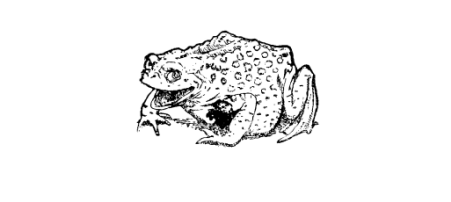
\includegraphics[scale=.5]{Toad}
  \end{center}



\SPELL[
  Name=Fool's Fire,
  Link=wizardry-fools-fire,
  Paradigm=Entropy,
  Save=Y (negate),
  Duration=Concentration,
  Counter=\mylink{Enervate}{wizardry-enervate} ,
  Keywords=Splittable,
  Target=Close or Nearby point
]



You project \DICE will-o'the-wisps into an area Close or Nearby.  The wisps
can move one range (Close to Nearby, Nearby to Far Away, etc) each Moment
for as long as you concentrate.  You can split the wisps up any way you like
but they can't be more than Far-Away from you.  The wisps do not shed heat,
do not require air, and can't be doused by water.  They shed a steady yellow
light the brightness of a torch.  At the top of the Moment, you can command
up to \DICE wisps to Befuddle up to \DICE Monsters that are Close to them.  The Befuddle affect lasts as long as you concentrate. 
The Monsters immediately get a Save to negate (one for each wisp that's targeting them), but a successful Save does not end the spell.  
If any of the wisps are struck by an Enervate spell, they are all dispelled if a Wizards' Duel is lost.  When a wisp is dispelled, any Monsters
Befuddled by the wisp are released from the effect.



\SPELL[
  Name=Greaseball,
  Link=wizardry-greaseball,
  Paradigm=Entropy,
  Save=N,
  Duration=Markovian,
  Counter=\mylink{Pritchard's Gusty Belch}{wizardry-pritchards-gusty-belch} (acid) ,
  Keywords=None,
  Target=Close or Nearby Monster or Object
]



Toss a small ball of grease at a point on the ground Close or Nearby. If you
would prefer to throw the ball at a person or object, make a Fight \RO using
your \INT - if you miss, it dissipates.  If thrown at the ground, the
surface becomes slick with a thick oil; anyone attempting to move through
the area must \RO using \DEX+\MD with a -\DICE penalty or immediately fall
Prone.  It requires a successful \RO as above to get up again.  If you throw it at a
creature, the effect is as above, plus they can't hold anything without
dropping it.  If you throw it at an object, the object becomes impossible to
carry or hold until the grease is removed with a mild or strong acid. 
Pritchard's Gusty Belch (acid variety) will dispel the grease if a Wizards'
Duel is lost.  The grease is highly flammable.  





\SPELL[
  Name=Grimm's Electric Fingers,
  Link=wizardry-grimms-electric-fingers,
  Paradigm=Elements,
  Save=Y (half),
  Duration=0,
  Counter=None ,
  Keywords=None,
  Target=Close or Nearby Monster or Object
]



Forks of lightning erupt from your outstretched hands, striking a Close or
Nearby target for \SUMDICE damage (Save for half). You can cause the
lightning to "jump" up to \DICE-1 times to another creature or object Close
by, provided they are conductive (iron armor, metal ladders, etc).  Magic
swords aren't conductive.  You can "ping-pong" between two objects if you
desire. Creatures struck by any bolt after the first take \DICE damage
(no Save). Objects struck by subordinate bolts will become
momentarily electrified, and deal a shock that could cause someone to lose
their grip unless they \RO : \VIG + \FOC with a -\DICE penalty.



\SPELL[
  Name=Hammerspace Mule,
  Link=wizardry-hammerspace-mule,
  Paradigm=Force,
  Save=N,
  Duration=Session,
  Counter=\mylink{Illusion}{wizardry-illusion} ,
  Keywords=Hammerspace,
  Target=Close
]



You create a spectral mule out of pure Force. The mule carries two
magical saddlebags that can each hold \SUMDICE Significant Items whose
combined weight doesn't exceed \DICE x 200kg (a reminder that a person is 25
Significant Items, and small creatures are 15).  The mule walks at a brisk
trot.  It will stop and turn at your verbal command, but you cannot make it
reverse or slow down. You can only give it the commands "go", "stop",
"left", and "right". If the mule takes any damage, it immediately disappears
and drops all the items on the ground.  The mule will obey your last command
until the spell's duration expires.  Hammerspace Mules think that Illusions
are real; if the Illusion would damage them in some way (a pit they would
fall into, a spear they would run into, etc) the Mule is dispelled (dropping
its items on the ground) if a Wizards' Duel is lost.





\SPELL[
  Name=Helping Hand,
  Link=wizardry-helping-hand,
  Paradigm=Biomancy,
  Save=N,
  Duration=Concentration,
  Counter=\mylink{Web}{wizardry-web} ,
  Keywords=None,
  Target=Self
]



You can detach either hand from its wrist.  The
hand floats at chest height and can hold anything you could normally hold. 
The hand can't use any weapons except for an Ego Weapon.  It can grab
shirts, press buttons, and shove people (but not too hard).  If anyone
attacks the hand, you have to roll your Guard as if they were attacking you. 
If your hand takes any damage, it disappears for the rest of the Session. 
Additionally, if the Hand is ever caught in a Web spell, it will disappear
if a Wizards' Duel is lost.  At the end of the Session, roll a d6.  If you roll a 1, your hand comes back 
as something else (a claw, a tentacle, etc) at the Arbiter's discretion - 
otherwise, it returns as normal.



\SPELL[
  Name=Heroic Leap,
  Link=wizardry-heroic-leap,
  Paradigm=Biomancy,
  Save=N,
  Duration=0,
  Counter=None ,
  Keywords=None,
  Target=Self or Close Ally
]



You and up to \DICE-1 allies can leap \VIG+\SUMDICE meters high and/or
\VIG+\SUMDICE meters forward in a straight line.  You take no damage on
landing, provided you land on or above the level you started from. For
example, you could leap from the ground to top of a steeple, or you could
leap over the steeple to land on the ground, but you couldn't leap from the
top of a steeple to the ground.  When you land, you can make a \RS : \DEX
(\RS : \INT if you are the caster) and if you succeed,
you can leap again. You can do this up to \DICE times.  You can't cast
spells or Fight while you're jumping around.





\SPELL[
  Name=Hollow Head,
  Link=wizardry-hollow-head,
  Paradigm=Biomancy,
  Save=N,
  Duration=Session,
  Counter=None ,
  Keywords=Hammerspace,
  Target=Self
]



You brain disappears and your head has a hinge that opens like a box, but
only you know this and only you can open it. For the rest of the Session,
you are immune to the next \DICE spells from the Mind paradigm, and you can
fit up to \SUMDICE Significant Items inside of your head in Hammerspace
(pulling one of these items out takes a Maneuver).  When you resist the
final Mind paradigm spell, the enchantment immediately ends. If the spell
ends while items are stored in your head they will mix with your
brain-matter. Usually this is fatal, though ambitious sorcerers sometimes
add drugs.  While your head is hollow, another sorcerer could read the
spell(s) inscribed on the inside.


  \begin{center}
  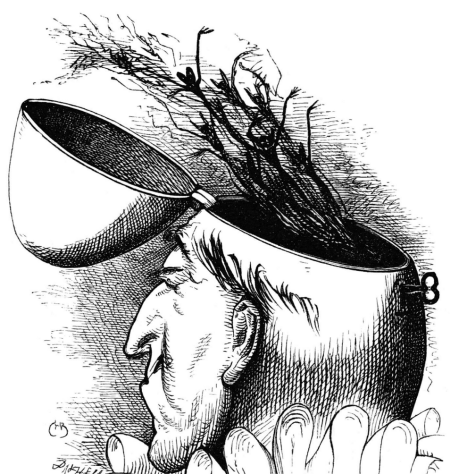
\includegraphics[scale=.5]{HollowHead}
  \end{center}





\SPELL[
  Name=Ice Bridge Step,
  Link=wizardry-ice-bridge-step,
  Paradigm=Elements,
  Save=N,
  Duration=Session,
  Counter=\mylink{Greaseball}{wizardry-greaseball} ,
  Keywords=None,
  Target=Self
]



You and up to \DICE-1 allies can run over liquids as if they were land.  Ice
forms beneath your feet with each step. If you slow down (to walk, fight,
etc), you'll sink. Very wavy seas may require you to \RS : \DEX.  Very hot
liquids (like lava) may require you to \RS : \INT.  The ability is dispelled
if you are struck by a Greaseball spell and you fail a Wizards' Duel.





\SPELL[
  Name=Icebolt,
  Link=wizardry-icebolt,
  Paradigm=Elements,
  Save=Y (half),
  Duration=0 / Markovian,
  Counter=None ,
  Keywords=None,
  Target=Close or Nearby point (straight line)
]



Throw a bolt of ice at a target Close or Nearby.  The bolt will travel in a
straight line from your fingers.  Anything touched by the bolt takes
\SUMDICE damage, Save for half.  Additionally, everything that fails its
Save is frozen to whatever surfaces they are touching.  Keys are frozen in
locks; swords are frozen to hands; boots are frozen to the ground
(creatures are usually immobilized from the boots down unless they were
playing in a fountain or something).  The objects are stuck until the
for a Markovian duration, based on the number of \DICE used.




\SPELL[
  Name=Illusion,
  Link=wizardry-illusion,
  Paradigm=Mind,
  Save=N,
  Duration=Varies,
  Counter=\mylink{Ego Weapon}{wizardry-ego-weapon} ,
  Keywords=None,
  Target=Varies
]



You create an illusion of anything you desire. If anything touches the
illusion, it will pass through it with no effect.  The illusion cannot be
greater than \DICE x \DICE meters in size.  Think of the illusion as a
perfectly accurate hologram that you are creating - the illusion can be
heard in addition to being seen, can perform the same action over and over
again, and can deliver messages, but it can't interact in a meaningful way
or perform complex actions based on external forces. 

Each aspect of the illusion requires one or more Blood die to cast:

\mylist {
  \item You want the illusion to say up to \DICE + \DICE words or make \DICE
+ \DICE sounds (wailing, shouting, etc)
  \item You want the illusion to be a physical thing (hole in the ground,
stone wall, orc guard, etc)
  \item You want the illusion to be able to move up to \DICE meters
  \item You want to cast the illusion on a living creature (disguise them as
a beggar or a lamp post)
}

Note that there is some Arbiter's discretion here.  A guard pacing in front
of a door might cost 2 \DICE (a physical thing moving back and forth 2
meters), but if you want the illusion of acrobats or pouncing lions it will
be more costly.  A disguise cast on someone to appear to be a beggar might
cost 1 [die] (a living creature wearing the face and clothing of a random
beggar), but disguising yourself as the king will be significantly harder.

The Illusion will last for \DICE Hours.  Anyone touching the illusion will
immediately know it to be fake, but this doesn't cause the illusion to
disappear.  However, if the illusion is touched with an Ego Weapon, it will
disappear if a Wizards' Duel is lost.





\SPELL[
  Name=Invisibility,
  Link=wizardry-invisibility,
  Paradigm=Entropy,
  Save=N,
  Duration=Varies,
  Counter=\mylink{Fool's Fire}{wizardry-fools-fire} ,
  Keywords=None,
  Target=Self or Close Allies or Objects
]



Up to \DICE objects or creatures can be made invisible (including yourself),
and will remain that way as long as they don't move.  As soon as the
creature or object moves (or is moved), the charm is broken.  Invisible
creatures can see other invisible and hidden objects (including Knaves using Whispers).  If this spell is cast on something Invisible, it will force the
object to become seen.  The duration of the charm depends on the dice
invested.  1 [die]: \SUMDICE Moments; 2 \DICE: Minutes; 3 \DICE: Hours; 4
\DICE Days; 5 \DICE: Weeks; 6+ \DICE: Forever.  The wisps from a Fool's Fire
can dispel the Invisibility of a Wizards' Duel is lost.

  \begin{center}
  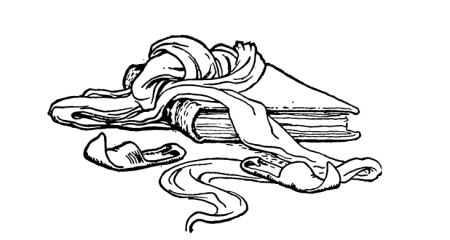
\includegraphics[scale=.5]{Invisibility}
  \end{center}





\SPELL[
  Name=Kelsier's Swarm of Irritating Vermin,
  Link=wizardry-kelsiers-swarm-of-irritating-vermin,
  Paradigm=Force,
  Save=N,
  Duration=Markovian,
  Counter=\mylink{Mighty Lungs}{wizardry-mighty-lungs} ,
  Keywords=None,
  Target=Close; Nearby; Far Away
]



You summon a cloud of tiny, magical, irritating vermin to an area Close,
Nearby, or Far-Away.  The vermin deal \DICE damage per Moment to every
living creature Close to them, but no damage to nonliving creatures or
objects. At the top of each Moment they are in the cloud, a non-mindless
creature must Save or take a -\DICE penalty on their Fight roll.  The vermin
won't move from the spot where they are summoned, and will remain until the
spell expires.  If the target is an object, the vermin will do minor
cosmetic damage, such as chewing holes in paper, gnawing wood, chipping
paint, and scratching glass.  Mighty Lungs will dispel the swarm if a
Wizards' Duel is lost.



\SPELL[
  Name=Knife Trick,
  Link=wizardry-knife-trick,
  Paradigm=Force,
  Save=N,
  Duration=Session,
  Counter=\mylink{Grimm's Electric Fingers}{wizardry-grimms-electric-fingers} ,
  Keywords=Splittable,
  Target=Close; Nearby; Far Away
]



Up to \DICE daggers orbit your head like a halo or crown.  These must be
daggers in your possession.  Magic and silver daggers are OK, as are other
"dagger-like" items (icicles, shards of glass, etc) at the Arbiter's
discretion.  At any time during the Session, you can mentally "throw" one or
more of these daggers at things that are Close, Nearby, or Far-Away with
unerring accuracy.  This could be used to sever a rope or pin something to a
wall (or stick into someone's chest) - but no Gambits, that wouldn't be
fair.  Each dagger does \SUMDICE+\DICE damage i.e. if you were to throw 1
dagger at someone, it would do d6+1, two daggers 2d6+2, etc.  Grimm's
Electric Fingers will dispel the magic and cause the daggers to fall to the
ground if a Wizards' Duel is lost.





\SPELL[
  Name=Knock,
  Link=wizardry-knock,
  Paradigm=Entropy,
  Save=N,
  Duration=0,
  Counter=\mylink{Lock}{wizardry-lock} ,
  Keywords=None,
  Target=Close or Nearby Objects
]



\DICE Close or Nearby object(s) is/are opened. Doors are flung wide, locks
are broken, shackles are bent open, belts come undone.  Ideas or thoughts
can be unlocked from a mind if a \RB : \INT contest is lost. Objects locked
by the Lock spell are opened if a Wizards' Duel is won.




\SPELL[
  Name=Levitating Disc,
  Link=wizardry-levitating-disc,
  Paradigm=Force,
  Save=N,
  Duration=Concentration,
  Counter=\mylink{Suspend Objects}{wizardry-suspend-objects} ,
  Keywords=None,
  Target=Close or Nearby point in space
]



You draw a circle in the air of \DICE+\DICE diameter, in any orientation. The inside of the
circle is made of Force, as solid as iron. You can cause the circle to
raise, lower, or hover in place.  You can only move up and down (never
side-to-side).  Up to \DICE people could stand under it and be completely
covered, or on it and be levitated provided they don't weigh more than \DICE
x200kg.  If you lower the circle on top of someone, they take \DICE damage
per Moment. The circle moves 10 meters a minute (about 3m per Moment).  You can change the disc's orientation
at any time.  If the Levitating Disc is targeted with Suspend Objects, the
disc will be dispelled if a Wizards' Duel is lost.





\SPELL[
  Name=Lipby Chonk's Viscous Form,
  Link=wizardry-lipby-chonks-viscous-form,
  Paradigm=Biomancy,
  Save=N,
  Duration=Combat or \SUMDICE Minutes,
  Counter=None ,
  Keywords=None,
  Target=Self
]



Your flesh becomes gelatinous. You can squeeze through gaps as small as a 
keyhole with a great deal of effort. You take no damage from Crushing
attacks for the duration of the spell. The spell only affects your flesh,
not anything you're wearing or carrying.




\SPELL[
  Name=Lock,
  Link=wizardry-lock,
  Paradigm=Mind,
  Save=Y (negate),
  Duration=Markovian,
  Counter=None ,
  Keywords=None,
  Target=Close and Nearby Objects
]



Up to \DICE non-living thing slam shut and can't be opened. If the object is
a door, chest, or something like it, it will slam shut forcefully and
loudly. This spell can work on things that aren't portals (a sword could be
locked in its scabbard). You can also use this spell to lock a specific
memory or thought, making it immune to mind reading or scrying without a \RB
: \INT try.  The duration is Markovian and depends on the number of
\DICE invested.  The Lock can be dispelled by the Knock spell if a Wizards'
Duel is lost.


\SPELL[
  Name=Meat Shield,
  Link=wizardry-meat-shield,
  Paradigm=Biomancy,
  Save=N,
  Duration=Combat or \SUMDICE Minutes ,
  Counter=None ,
  Keywords=None,
  Target=Close and Nearby
]

You summon a giant slab of meat.  The meat has \SUMDICE+\DICE Health, and
can fill an area \DICE meters cubed.  The meat weighs \DICE x100kg and lasts
for \DICE Hours.  Zoological creatures will attack the Meat Shield first. 
Up to \DICE other creatures can eat the Meat Shield in lieu of rolling their
Provisions, but the provenance of the meat is ... unknown.  If a Scything
Disc of Nog is used on a Meat Shield, the shield will be dispelled if a
Wizards' Duel is lost (otherwise, it will take damage as normal).





\SPELL[
  Name=Mighty Lungs,
  Link=wizardry-mighty-lungs,
  Paradigm=Biomancy,
  Save=N,
  Duration=Until exhalation,
  Counter=None ,
  Keywords=Contested,
  Target=Self
]

Your next inhalation allows you inhale 10x the normal amount of air. Not
only does this allow you to hold your breath for 10x as long, but if you
exhale forcefully it will release a blast of air strong enough to knock
pigeons out of air and polish your teeth. A human-sized creature is knocked
Prone and pushed Nearby unless they try a \RB: \DEX or \VIG
(their choice) with a -\DICE penalty vs your \INT.  This spell will also blow open all
closed but unlocked doors in a room, shatter all windows in a
building, or knock the thatched roof off a peasant's shack. If you cast this
spell with 3 or more \DICE, Save or your teeth shatter.




\SPELL[
  Name=Mirror Image,
  Link=wizardry-mirror-image,
  Paradigm=Entropy,
  Save=N,
  Duration=Combat or \SUMDICE Minutes,
  Counter=None ,
  Keywords=None,
  Target=Self
]



You create \DICE illusory images of yourself, which move as you move and
always stay Close to you. They are constantly stepping through each other,
so that it is impossible to tell which is which. When an enemy attacks you,
they'll always hit an image first.  An image vanishes as soon as it suffers
a solid impact (a blow from a mace, but also a slap). Area effects such as a
dragon's breath will cause all images to instantly vanish (and you take the
damage, naturally).





\SPELL[
  Name=Morass,
  Link=wizardry-morass,
  Paradigm=Elements,
  Save=N,
  Duration=Concentration,
  Counter=\mylink{Bastogne's Glamping Charm}{wizardry-bastognes-glamping-charm} ,
  Keywords=Contested,
  Target=Nearby or Far-Away Area
]



The ground \SUMDICE meters in radius and \DICE meters deep turns to black
muck.  Monsters and objects in the mud sink 1 meter per Moment.  At the top of
the Moment, a creature can \RB: \VIG with a -\DICE penalty vs. your \INT 
to pull themselves out 1 meter (if they were only 1 meter deep to
begin with, they escape).  If someone's head dips below the mud (2m for
people, 1m for Pooka, 4m or more for giants), they immediately being drowning and must make a \DEATH 
roll at the top of every Moment they are submerged (they can still claw their way up 1m with a successful \RB try,
as above).  If they don't have a \DEATH, they die in \HD Moments.

The spell lasts for as long as you concentrate.  When you break your
concentration, everything that sunk in the mud is immediately vomited back to
the surface.   If the area covered by the Morass is targeted by Bastogne's
Glamping Charm, the Morass will be dispelled (and the objects brought to the
surface) if a Wizards' Duel is lost.




\SPELL[
  Name=Negasonic Bomb,
  Link=wizardry-negasonic-bomb,
  Paradigm=Mind,
  Save=N,
  Duration=Concentration,
  Counter=\mylink{Cacaphony}{wizardry-cacaphony} ,
  Keywords=None,
  Target=Nearby or Far Away Area
]



You roll a small orb of Mind to a point Close, Nearby or Far-Away; the orb
rolls silently and is hard to see.  When the orb stops rolling it
immediately and silently detonates.  Creatures Close to the designated point
are Deafened until they leave the area of effect.  Likewise, no spells can
be cast while Close to the Negasonic Bomb.  Murder attempts against anyone deafened in this way succeed automatically. The spell lasts as long as
you concentrate.  The bomb can be dispelled by Cacaphony if a Wizards' Duel
is lost.





\SPELL[
  Name=Prismatic Ray,
  Link=wizardry-prismatic-ray,
  Paradigm=Entropy,
  Save=Y (half),
  Duration=0,
  Counter=None ,
  Keywords=Splittable,
  Target=Nearby or Far-Away
]



A brilliant white light emanates from your forehead to a point Nearby or
Far-Away, where it splits into a prism of \DICE beams.  Each beam strikes a
random Ally or Monster Close to the prism.  Roll a d8 on the table below for
each beam and apply its results.

\mynumlist {
  \item \mybold{Red} Target takes \DICE fire damage, Save for half. Highly flammable things catch fire.
  \item \mybold{Orange}  Target takes \DICE bashing damage, Save for half. 
  \item \mybold{Yellow} Target takes \DICE lightning damage, Save for half.  If you fail your Save, you drop what you're holding.
  \item \mybold{Green} Target takes \DICE acid damage, Save for half. Roll your Armor \UD if applicable.
  \item \mybold{Blue} Target takes \DICE ice damage, Save for half. If you fail your Save, you fall Prone.
  \item \mybold{Indigo} Target takes \DICE stabbing damage, Save for half.
  \item \mybold{Violet} Target takes \DICE chopping damage, Save for half.
  \item \mybold{Roll} again.  Instead of \DICE damage, the effect deals \SUMDICE damage.. If you get this result again, the beam splits and the target takes an additional effect (roll again and apply the result).  Continue in this way until you don't roll an 8.
}





\SPELL[
  Name=Pritchard's Gusty Belch,
  Link=wizardry-pritchards-gusty-belch,
  Paradigm=Biomancy,
  Save=N,
  Duration=0,
  Counter=None ,
  Keywords=None,
  Target=Close and Nearby Area
]



You can breathe out up to \DICE elements (fire, acid, water, wind, steam, etc)
immediately in front of you for a Moment.  The elements don't interact with
one another and act independently, so if you were to belch out fire and
water, you would get the effects of both.  If the order matters (set
something on fire and immediately douse it with water), you pick the order
of effects.  Water breath is enough to extinguish fires smaller than a big
bonfire, or wash off acid; wind breath could push a small sailboat or blow
swarming insects out of an area; acid breath bleaches the color from objects
and irritates the eyes; fire breath would cause paper and flammable objects
(but not people, unless they were doused in oil) to catch fire, etc.




\SPELL[
  Name=Protection from Element,
  Link=wizardry-protection-from-element,
  Paradigm=Elements,
  Save=N,
  Duration=Session,
  Counter=\mylink{Prismatic Ray}{wizardry-prismatic-ray} ,
  Keywords=Splittable,
  Target=Self or Close Allies
]



Reduce all damage of a single chosen element (acid, cold, fire, lightning,
etc) by -\DICE.  The spell protects its targets from the negative effects of
the natural elements (desert heat, arctic chill) as well.  If you are struck
by a Prismatic Ray of the same elemental type, the protection is dispelled
if a Wizards' Duel is lost.


  \begin{center}
  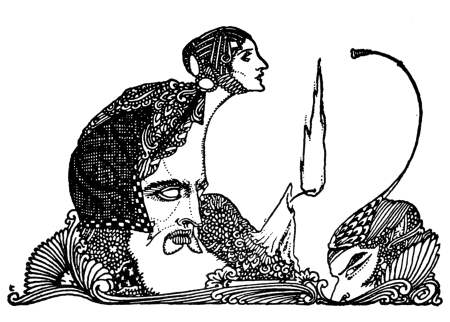
\includegraphics[scale=.5]{Wizardry_1}
  \end{center}



\SPELL[
  Name=Rhea's Efficacious Plow,
  Link=wizardry-rheas-efficacious-plow,
  Paradigm=Force,
  Save=N,
  Duration=Moments,
  Counter=None ,
  Keywords=None,
  Target=See description
]



You send an invisible wedge of Force along the ground in a straight line up
to a Distant point.  The wedge can take up to \DICE turns ("left" or
"right") at your command.  Any light debris on the path (snow, small stones,
leaves, grass) is pushed to the side; fields can be tilled. Any pressure
plates or tripwires are activated. You do not have to be able to see the
entire path, but you do need to know the approximate route the wedge will
take. The wedge can't move through solid objects, and it can't hurt anyone (though it will push them to the side).
The path cleared is \DICE meters wide. If you cast this spell with 3 \DICE
or more, the width becomes \SUMDICE meters wide.




\SPELL[
  Name=Sandstorm,
  Link=wizardry-sandstorm,
  Paradigm=Elements,
  Save=N,
  Duration=Concentration,
  Counter=None ,
  Keywords=None,
  Target=Close
]



You cough up a swirling spiral of sand.  Small flying creatures (bug-sized),
arrows, and spears cannot enter or leave the sandstorm.  Up to \DICE-1 other
people can hide in the sandstorm with you.  The sand moves with you and
lasts as long as you concentrate.



\SPELL[
  Name=Sanguine Mail,
  Link=wizardry-sanguine-mail,
  Paradigm=Biomancy,
  Save=N,
  Duration=Session,
  Counter=\mylink{Enervate}{wizardry-enervate} ,
  Keywords=None,
  Target=Self
]



You become encased in elaborate plate mail that seems to be made from
constantly congealing blood.  You definitely stand out in a crowd. Your \MD
drops to d4, but you can still cast spells.  The \UD for the Armor depends
on the number of \DICE invested: 1 d3; 2 d4; 3 d6; 4 d8; 5 d10; 6+ d12.  If
you are struck with an Enervate spell, the Sanguine Mail is dispelled if a
Wizards' Duel is lost.





\SPELL[
  Name=Scuttle,
  Link=wizardry-scuttle,
  Paradigm=Biomancy,
  Save=N,
  Duration=Combat or \SUMDICE Minutes,
  Counter=\mylink{Greaseball}{wizardry-greaseball} ,
  Keywords=None,
  Target=Self
]



Your clothes and hair animate to carry you around. You can move at full
speed in any orientation, and you can freely rotate as you move. For
instance, you could run while standing on your head, holding a torch, and
turning counterclockwise. You can lie on your side and, while flipping end
over end, move backwards. This effect does not allow you to climb up walls,
but ladders and ropes are no problem (you could suspend yourself from a rope
and cast spells, for example).  If you are struck with a Greaseball, or
attempt to climb something affected by Greaseball, the Scuttle is dispelled
if a Wizards' Duel is lost.




\SPELL[
  Name=Scything Disc of Nog,
  Link=wizardry-scything-disc-of-nog,
  Paradigm=Force,
  Save=Y (half),
  Duration=0,
  Counter=None ,
  Keywords=None,
  Target=Nearby or Far Away Area
]



You hurl a whirling disc of Force and light from your fingertip. The disc
screeches like a sawblade. It deals \SUMDICE damage to its target, Save for
half. If it deals more than 6 damage, it bounces towards a random creature
(friend, foe, or even yourself) Close or Nearby, dealing \SUMDICE-2
damage, Save for half. If it deals more than 6 damage, it bounces towards
another random creature Close or Nearby, dealing \SUMDICE-4 damage, Save for
half. This continues, losing 2 damage with each bounce, until there are no
valid targets or the spell deals 6 or less damage to a creature.





\SPELL[
  Name=Sleep,
  Link=wizardry-sleep,
  Paradigm=Mind,
  Save=Y (negate),
  Duration=Markovian,
  Counter=\mylink{Cacaphony}{wizardry-cacaphony} ,
  Keywords=None,
  Target=Close or Nearby Area
]



You summon a cloud of somnolent dust to a point Close or Nearby. 
\SUMDICE creatures Close to the cloud, who have no more than \DICE \HD, must
immediately Save or fall into a magical slumber.   They can't be awakened by
anything less than a vigorous slap (counts as a Maneuver).  You don't have
control over who falls asleep, it's entirely random and will be as many
creatures as possible (up to \SUMDICE).  You are immune to your own Sleep
spell (so you could cast it Close to yourself).  Creatures who fall asleep
immediately fall Prone and drop any items they're holding.  Fight rolls
against them will hit automatically and do maximum damage, and can only be
blocked by Armor.  This will wake the creature up, of course.  If an orb of
Cacaphony is detonated Nearby, the creatures will awaken if a Wizards' Duel
is lost.  Otherwise, creatures who fall asleep will remain asleep for the
Markovian duration.   




\SPELL[
  Name=Summon Candles,
  Link=wizardry-summon-candles,
  Paradigm=Force,
  Save=N,
  Duration=Varies,
  Counter=\mylink{Fogbank}{wizardry-fogbank} ,
  Keywords=None,
  Target=Close
]



\SUMDICE dribbling candles appear on objects you touch. You can walk around
placing candles as required for Minutes. The candles are lit and burn for
Hours. They can be detached, but will fade from existence within Minutes. 
For every 6 candles placed Close to one another, the wizard close to the
candles gains 1 of the following (your choice): Safe Casting: Replace one of
your rolled Blood Die with a natural 1; Power Casting: Replace one of your
rolled Blood Die with a natural 6; Natural Casting: add a natural +1 to any
Blood Die you've rolled.  When you use 1 of these powers, the 6
candles immediately disappear.  Note that \myital{any} sorcerer can use these
abilities, friend or foe.  A philosopher will immediately know if they are in
an area of candles, and what powers it can bestow on them.  If the candles
are encased in a Fogbank, they are snuffed out and dispelled if a Wizards'
Duel is lost.





\SPELL[
  Name=Suspend Objects,
  Link=wizardry-suspend-objects,
  Paradigm=Force,
  Save=Y (negate),
  Duration=Concentration,
  Counter=\mylink{Levitating Disc}{wizardry-levitating-disc} ,
  Keywords=None,
  Target=Any Distance
]



You can hold up to \DICE objects in the air, weighing no more than \DICE
x200kg.  You can allow these objects to descend at 3m per Moment at your
discretion. Creatures who are brought to ground in this way take no falling
damage.  Unwilling creatures (flying Monsters, for example) get a Save to
negate.  If a Levitating Disc is summoned in the midst of the held
creatures, the Suspend Objects spell will be dispelled (and the objects will
fall) if a Wizards' Duel is lost.




\SPELL[
  Name=Tempestuous Chariot,
  Link=wizardry-tempestuous-chariot,
  Paradigm=Elements,
  Save=N,
  Duration=One trip,
  Counter=None ,
  Keywords=None,
  Target=Close
]



A tumult of air elementals lifts you and \DICE-1 others and takes you in any
direction the you desire, up to \SUMDICE km away.   One catch - the
elementals can only travel in a straight line, and you have to choose
beforehand the way to go ("up", "east", "that way", etc).  While you are in
the tempest you are buffeted horribly and can neither talk nor act.  The
winds refuse to travel without you, and will immediately dispel if you lose
contact




\SPELL[
  Name=Vertigo,
  Link=wizardry-vertigo,
  Paradigm=Mind,
  Save=Y (negate),
  Duration=Markovian,
  Counter=\mylink{Suspend Objects}{wizardry-suspend-objects} ,
  Keywords=None,
  Target= Any Distance
]



You can cause up to \DICE Close, Nearby, Far-Away, or Distant creatures to
suffer severe vertigo unless they Save.  Creatures that are climbing or
flying immediately fall; creatures who are Close to the edge of something (a
cliff, a wall, the guardrails of a ship, etc) need to \RS : \FOC or fall.
Creatures already on the ground will fall Prone.  If the creatures are
struck with a Suspend Objects spell, the Vertigo is dispelled if a Wizards'
Duel is lost.




  \begin{center}
  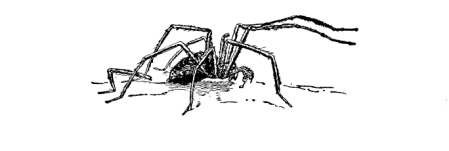
\includegraphics[scale=.5]{Spider}
  \end{center}


\SPELL[
  Name=Web,
  Link=wizardry-web,
  Paradigm=Entropy,
  Save=Y (negate),
  Duration=Markovian,
  Counter=None ,
  Keywords=None,
  Target=Nearby or Far Away Area
]



You can anchor a giant web between three or more solid points up to \DICE
meters in radius (for example: the 4 points of a door, two trees and the
ground, across a hallway, etc).  Objects that touch the web immediately
become stuck; arrows and spears can't be fired through it.  Creatures that
enter the web (or are caught in it when cast) must Save or become ensnared
for the Markovian duration (each creature should roll their Markovian die
separately). Fight rolls against them hit automatically and can only be
blocked by Armor.  The web is extremely flammable and will be consumed in
\DICE Moments.



\SPELL[
  Name=Whirling Blades,
  Link=wizardry-whirling-blades,
  Paradigm=Entropy,
  Save=N,
  Duration=Concentration,
  Counter=\mylink{Suspend Objects}{wizardry-suspend-objects} ,
  Keywords=None,
  Target=Self
]



You summon a number of invisible blades of Force that spin around your
waist, with you in the center.  Every creature Close to you takes \DICE
damage for each Moment the spell is maintained.  The blades will cut or
damage fragile objects.  If the creature or object sits above or below your
waist, they take no effect.  If the blades are struck by a Suspend Objects
spell, they will be dispelled if a Wizards' Duel is lost.



